\section{Risk \& Opportunity Management Process}
\label{sec:process}

This section describes the process by which risks and opportunities are managed during observatory operations.
Risks and opportunities are set to one of the statuses and follow the lifecycle described in Figure \ref{fig:risk-lifecycle}.

\begin{itemize}
	\item \textbf{Candidate} ---
	Risks and opportunities in a draft state, which are not actively managed by the project.

	\item \textbf{Active} ---
	Risks and opportunities deemed valid, and actively managed by the project.

	\item \textbf{Realized} ---
	Risks and opportunities which have been realized.
	There are three models available for the trigger:
		\begin{itemize}
			\item \textbf{Specific Trigger Date} ---
			A specific calendar date when contingency funds must either be obligated to respond to a risk, the risk can be retired, or an opportunity's beneficial event will occur.
			
			\item \textbf{Random Occurrence} ---
			Certain risks or opportunities are known to potentially occur but their date(s) are random; for example, critical staff may depart the project, weather delay, equipment failure.
			This type of event requires an estimate of the number of random occurrences and the cost of each.

			\item \textbf{Distributed Occurrence} ---
			Identical risks or opportunities are sometimes distributed throughout periods in the project; for example, software packages are evaluated for performance on an annual basis.
			This type of event distributes the possible contingency obligation profile over the specified time span.
		\end{itemize}

	\item \textbf{Retired} ---
	Risks and opportunities which can no longer valid or actively managed, as they have been realized or the event trigger can no longer occur.

	\item \textbf{Depreciate} ---
	Risks and opportunities that were deemed invalid and are were not actively managed.
\end{itemize}	

\begin{figure}[t]
\caption{Lifecycle of Risks.}
\centering
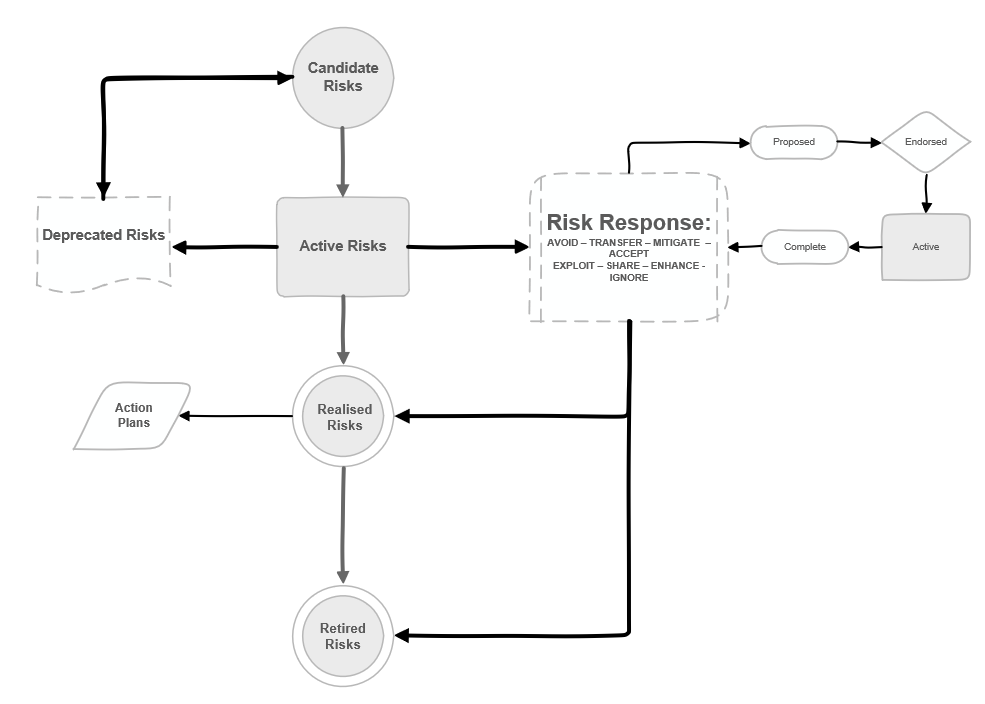
\includegraphics[width=\textwidth]{risk-lifecycle-temp}
\label{fig:risk-lifecycle}
\end{figure}
